\documentclass{beamer}

\mode<presentation>
{
  \usetheme{CambridgeUS}
  \setbeamercovered{transparent}
}

\usepackage[english]{babel}
\usepackage[latin1]{inputenc}
\usepackage{times}
\usepackage{amssymb}
\usepackage[T1]{fontenc} 
% Or whatever. Note that the encoding and the font should match. If T1
% does not look nice, try deleting the line with the fontenc.
\usepackage{amsmath}

\newcommand{\linespace}{\vskip 0.25cm}

\definecolor{MyForestGreen}{rgb}{0,0.7,0} 
\newcommand{\tableemph}[1]{{#1}}
\newcommand{\tablewin}[1]{\tableemph{#1}}
\newcommand{\tablemid}[1]{\tableemph{#1}}
\newcommand{\tablelose}[1]{\tableemph{#1}}

\definecolor{MyLightGray}{rgb}{0.6,0.6,0.6}
\newcommand{\tabletie}[1]{\color{MyLightGray} {#1}}

% The text in square brackets is the short version of your title and will be used in the
% header/footer depending on your theme.
\title[Mobile Security]{Improving Mobile Security}

% Sub-titles are optional - uncomment and edit the next line if you want one.
% \subtitle{Why does sub-tree crossover work?} 

% The text in square brackets is the short version of your name(s) and will be used in the
% header/footer depending on your theme.
\author[Luthi]{Braden Luthi}

% The text in square brackets is the short version of your institution and will be used in the
% header/footer depending on your theme.
\institute[U of Minn, Morris]
{
  Division of Science and Mathematics \\
  University of Minnesota, Morris \\
  Morris, Minnesota, USA
}

% The text in square brackets is the short version of the date if you need that.
\date[April '14, ] % (optional)
{29 April 2014 }

% Delete this, if you do not want the table of contents to pop up at
% the beginning of each subsection:
\AtBeginSection[]
{
  \begin{frame}<beamer>
    \frametitle{Outline}
    \tableofcontents[currentsection, hideothersubsections]
  \end{frame}
}

\begin{document}

\begin{frame}
  \titlepage
\end{frame}

% For a 20-25 minute senior seminar talk you probably want something like:
% - Two or three major sections (other than the summary).
% - At *most* three subsections per section.
% - Talk about 30s to 2min per frame. So there should probably be between
%   15 and 30 frames, all told.

\section*{Overview}


\subsection*{Outline}

\begin{frame}
  \frametitle{Outline}
  \tableofcontents[hideallsubsections]
\end{frame}
\section{Background}
\subsection{Cryptography}
 %----------------------- Cryptography Background ---------------------%
	\begin{frame}
	\frametitle{Cryptography}
	
		Cryptography or `secret writing' is the study and practice of techniques for securing communications between two parties. \linebreak
		\begin{itemize}
			\item \textbf{plain-text}  Readable message to be sent during communications.
			\item \textbf{cipher-text} Unreadable form of the message
			\item \textbf{key} parameter for cryptographic algorithm or cipher		
			\item \textbf{cipher} method for transforming plain-text
			\begin{itemize}
				\item \textbf{Encrypt} transform plain-text to cipher-text
				\item \textbf{Decrypt} transform cipher-text back into plain-text
			\end{itemize}
			%--add toy cipher example--%
		\end{itemize}		
		\textbf{Shift Cipher}\\

		\textit{``Hello World!''} $\underrightarrow{\text{Shift letters by 1}}$ \textit{``Ifmmp Xpsme!''} 
	%basic introduction to cryptography and vocabulary
	
	\end{frame}
	\begin{frame}
	\frametitle{Cryptography}
		\begin{itemize}
			\item \textbf{Symmetric cryptography} 
			Both parties share a secret key for encryption and decryption
			\item \textbf{Asymmetric cryptography}
			Each individual has a public and a private key. Parties use the public keys for encryption and the private keys for decryption
		\end{itemize}
		%--add Asymmetric example--%
	
	\end{frame}
 % ------------------- GSM and UMTS Background ---------------------------%
\subsection{GSM and UMTS}
	
		\begin{frame}
		\frametitle{GSM and UMTS}
		\begin{itemize}
		\item Global System for Mobile Communications (GSM) is a 2G telecommunication standard developed in the early 90s by the European Telecommunications Institute. Has become one of the most widely used standards, reaching an 80\% market share at its height.
					
		
		\item Universal Telecommunications Standard (UMTS) is 3G telecommunication standard based on GSM by the Third Generation Partnership Project in the early 2000s.   
		\end{itemize}
		%--Mention interworking networks here--%
	\end{frame}

	
\section{GSM Weakness in UMTS}

	

	\begin{frame}
	\frametitle{Encryption in GSM and UTMS}
	\begin{itemize}
	
	
		\item GSM and UMTS both have secret keys that are shared between the mobile and the mobile's home network authentication center.
		\item Keys in GSM are 64 bits
		\item Keys in UMTS are 128 bits
		
		\item GSM and UMTS both utilize the A5 family of encryption algorithms. 
		 \begin{itemize}
			\item A5/0 
			\item A5/1
			\item A5/2
			\item A5/3 
		\end{itemize}
		\end{itemize}
	\end{frame}
	
\subsection{Authentication}

%-----------GSM Authentication-----------------%
	% Talk Mention GSM weakness to Man in the middle Attack
\begin{frame}
% add hidden frames, introduce requests one at a time
  \frametitle{GSM Authentication}
  \begin{center}
  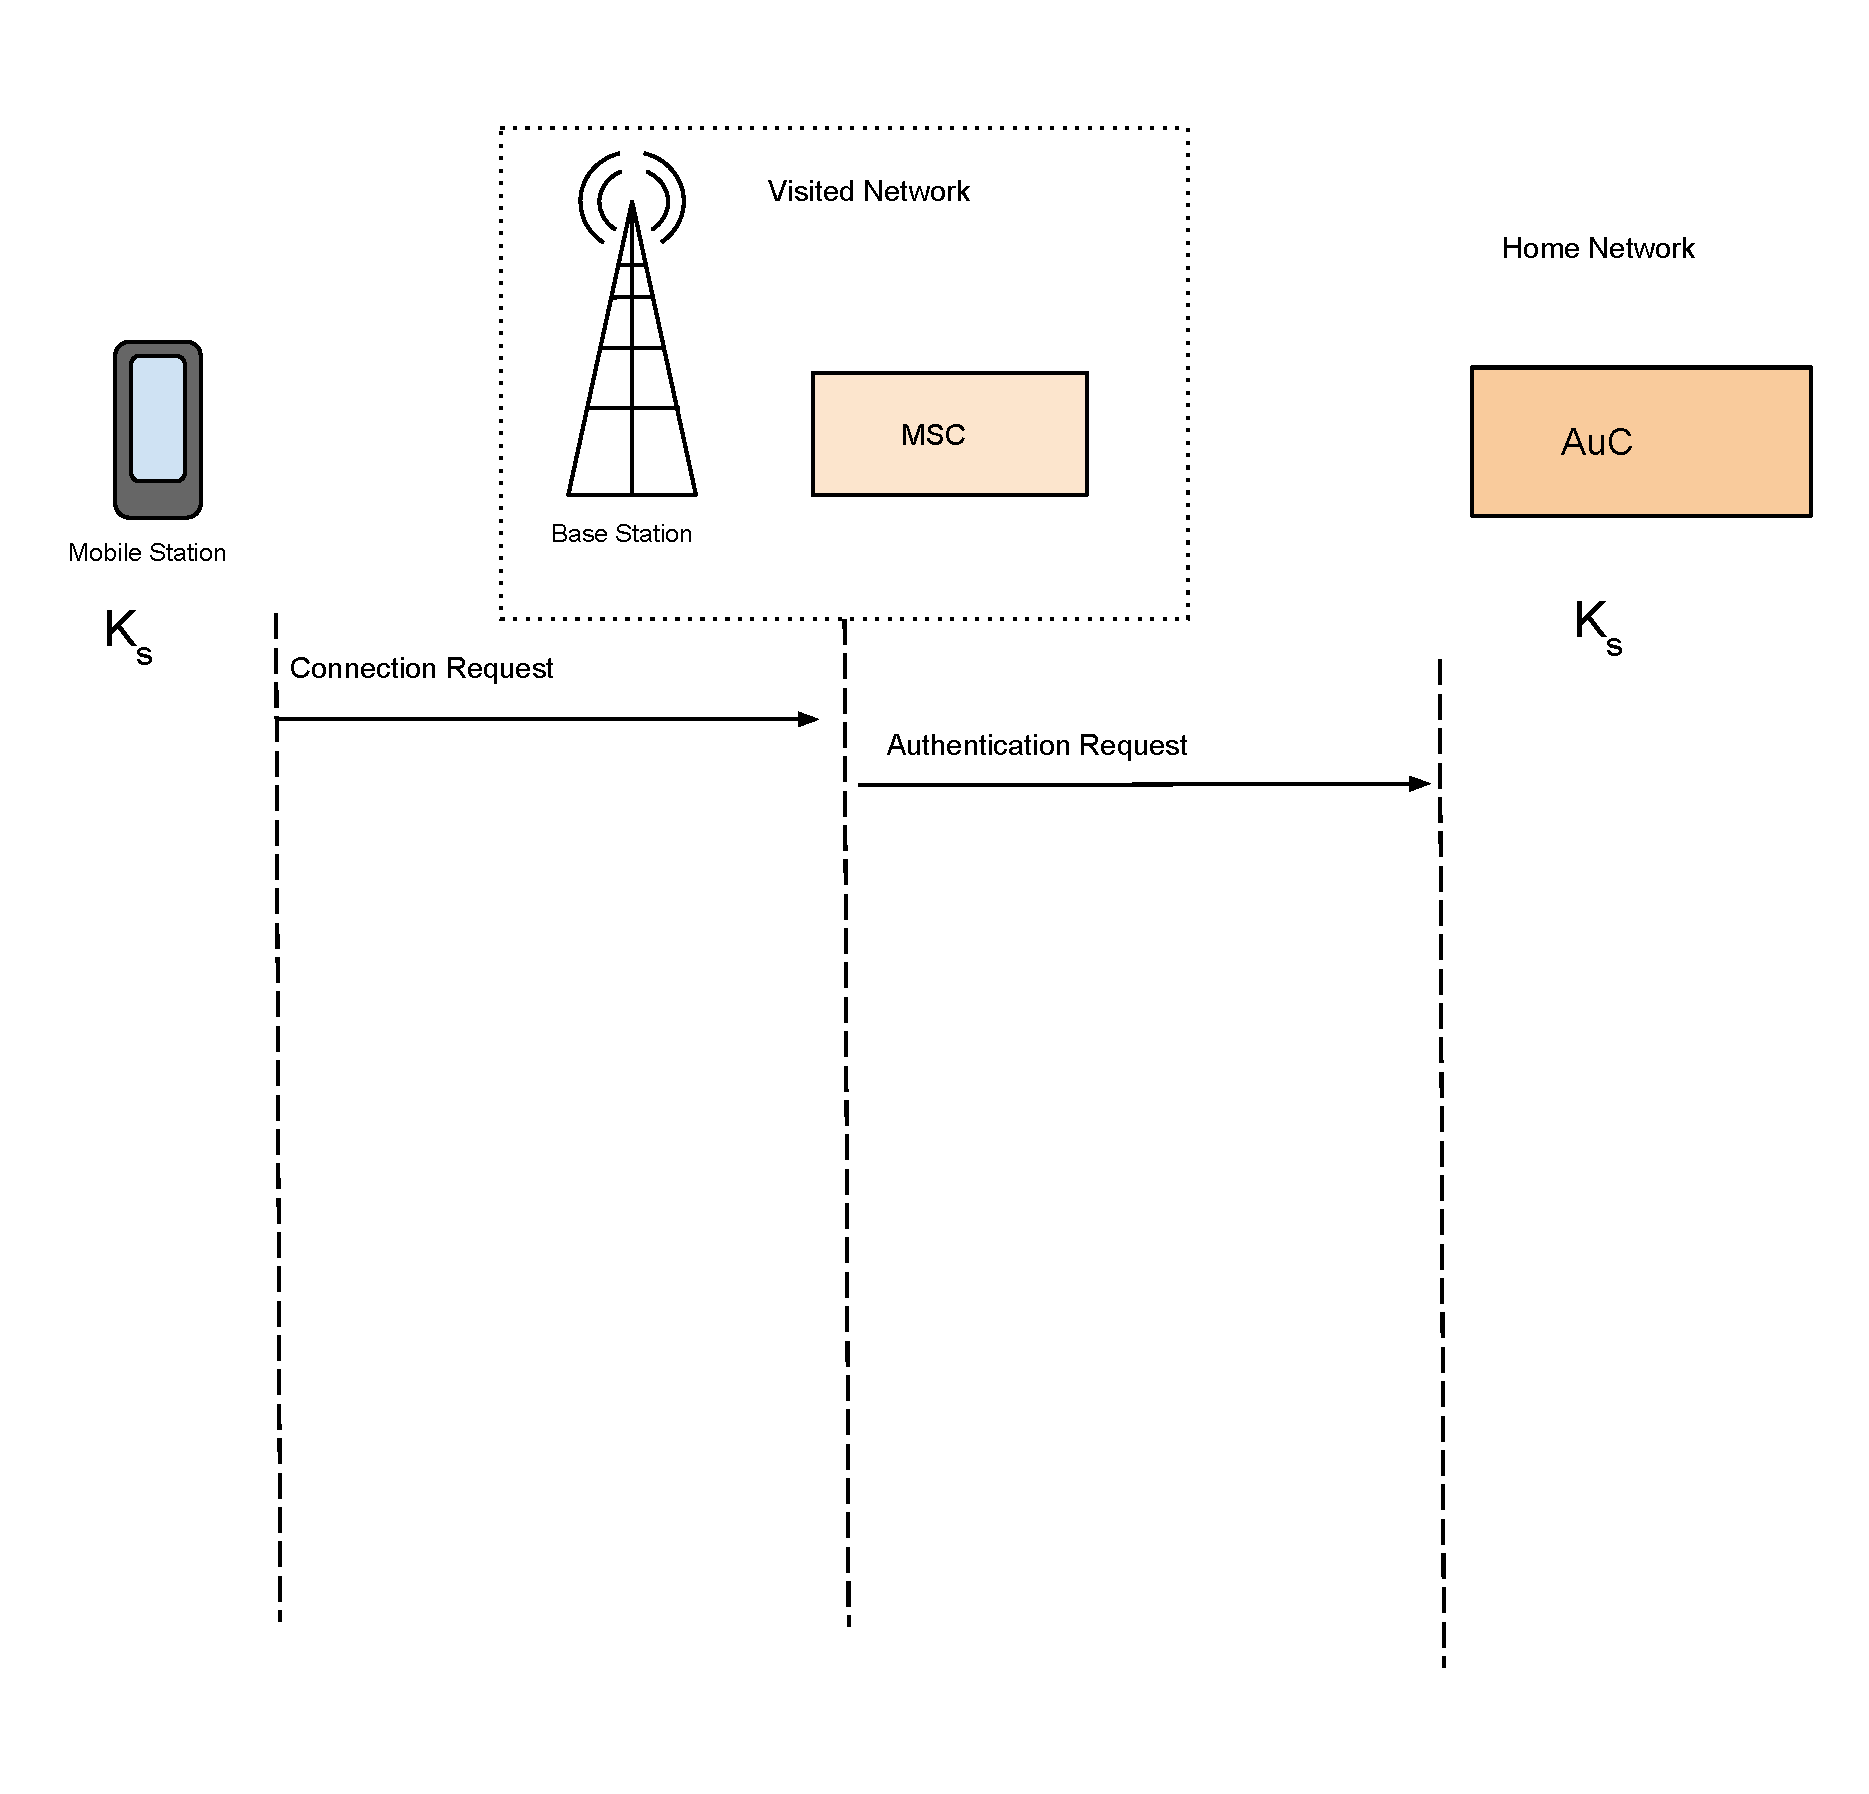
\includegraphics[width=.9\textwidth, height=.85\textheight]{Images/GSMAuthentication1.pdf}

  \end{center} 
\end{frame}
\begin{frame}
% add hidden frames, introduce requests one at a time
  \frametitle{GSM Authentication}
  \begin{center}
  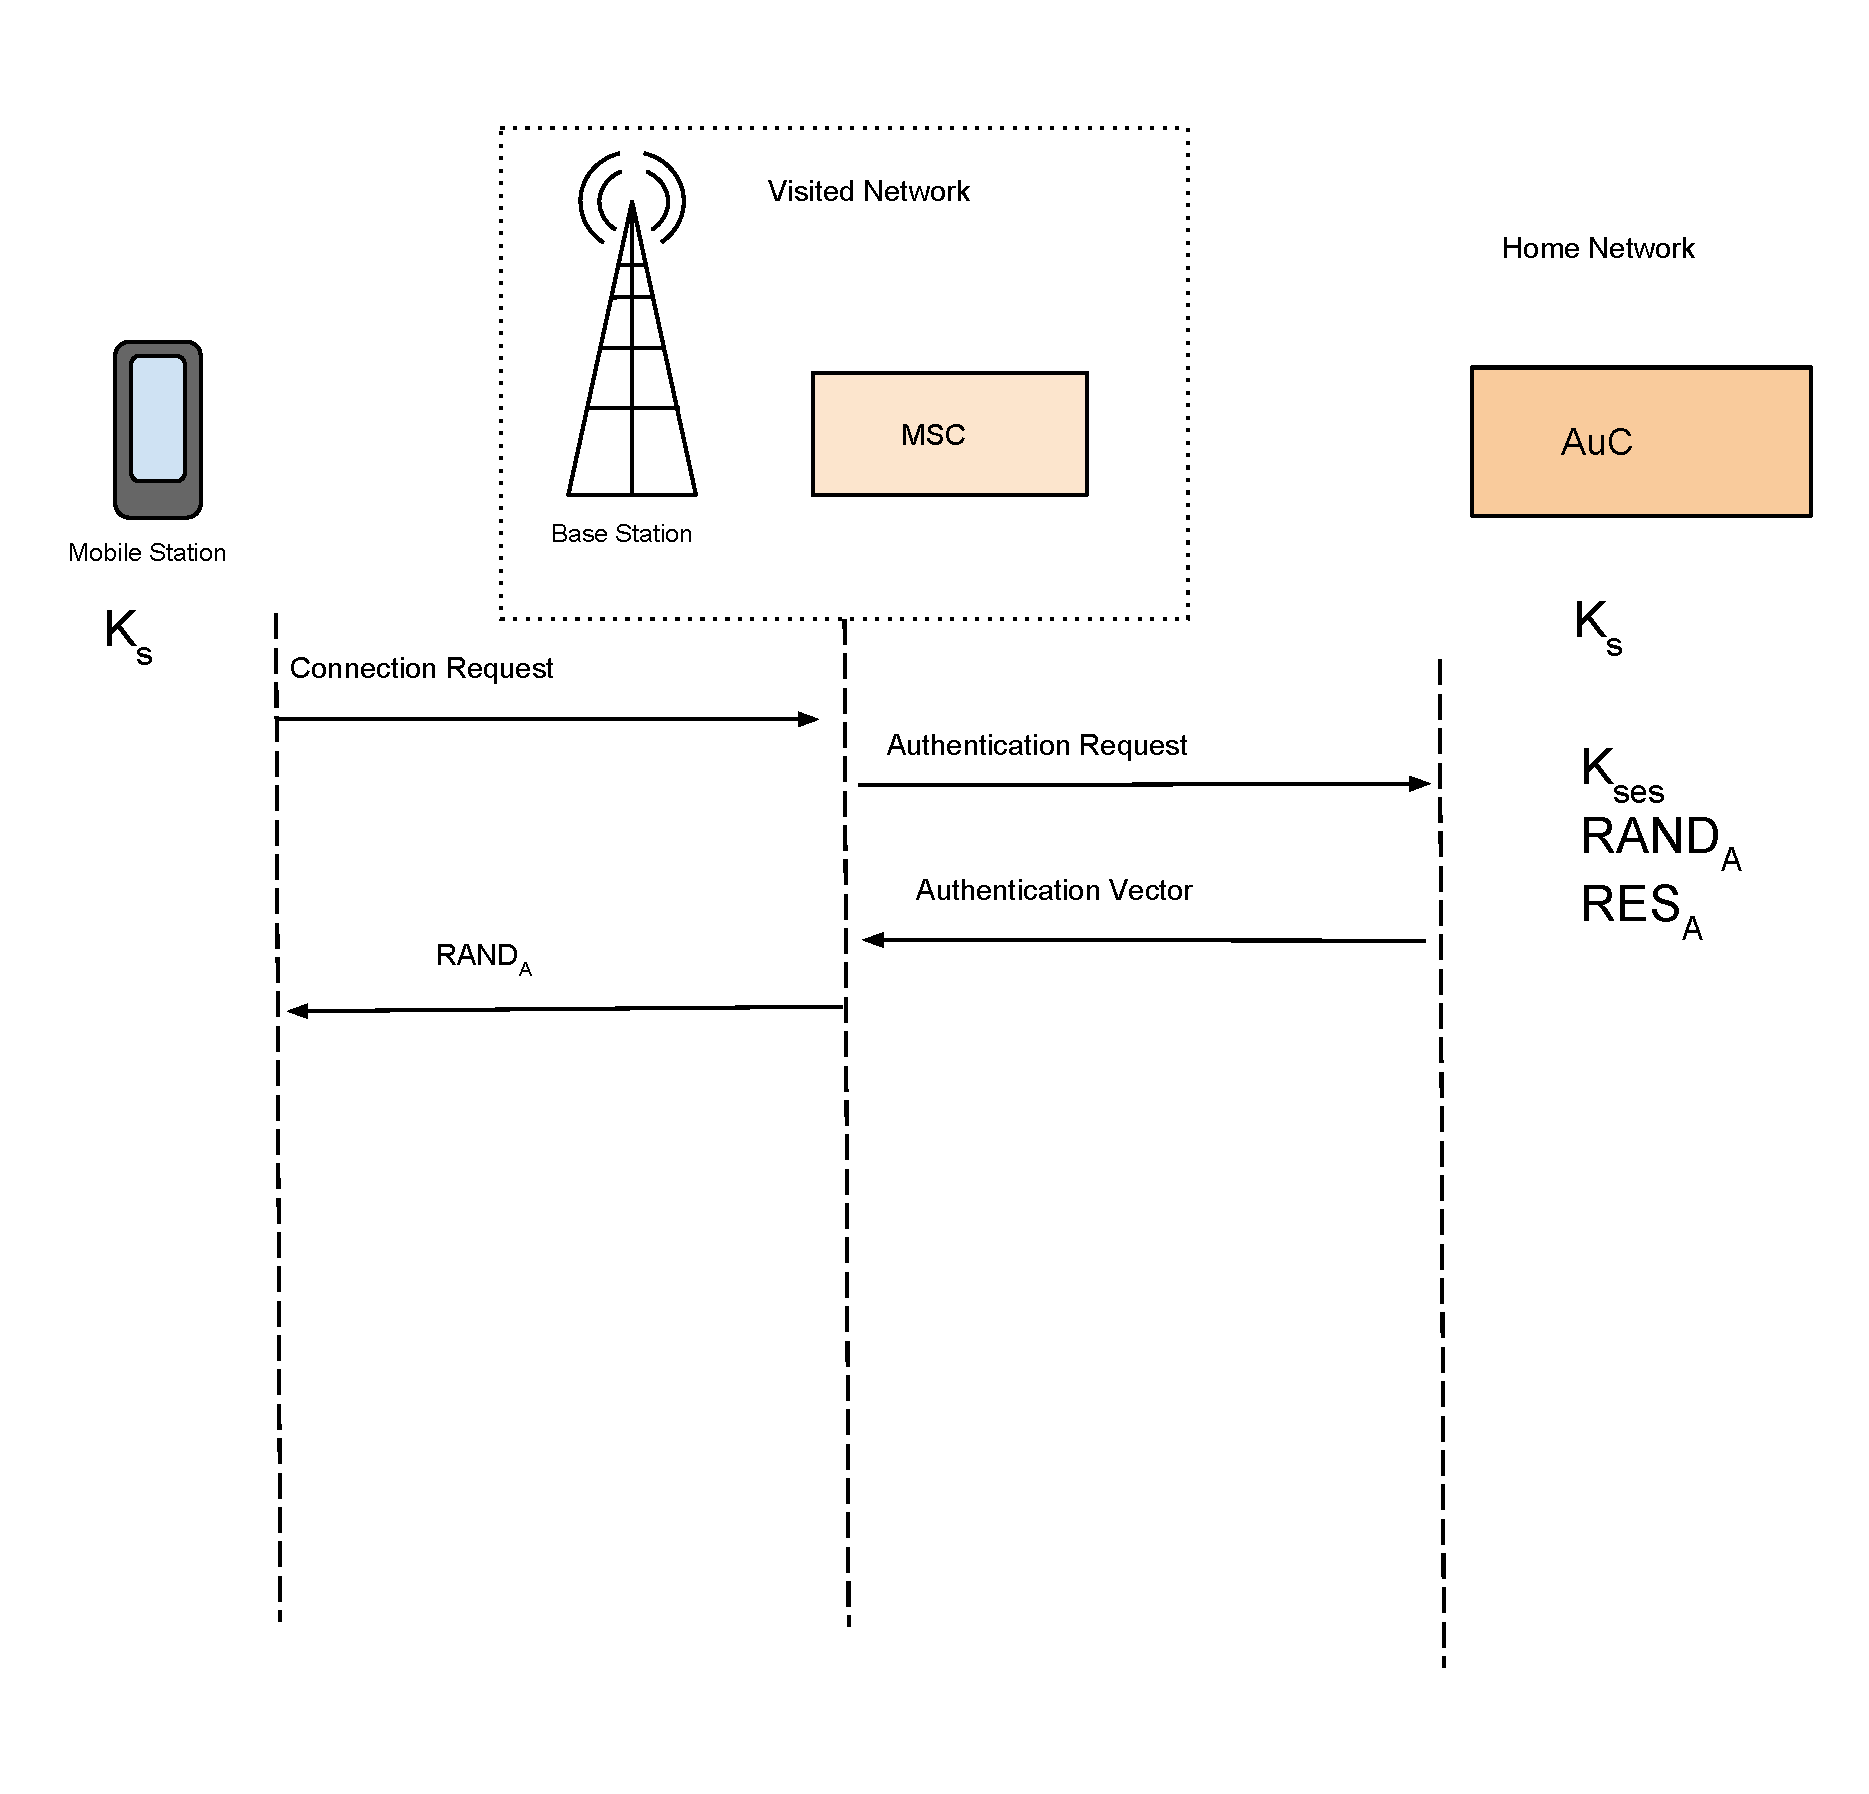
\includegraphics[width=.9\textwidth, height=.85\textheight]{Images/GSMAuthentication2.pdf}

  \end{center} 
\end{frame}
\begin{frame}
% add hidden frames, introduce requests one at a time
  \frametitle{GSM Authentication}
  \begin{center}
  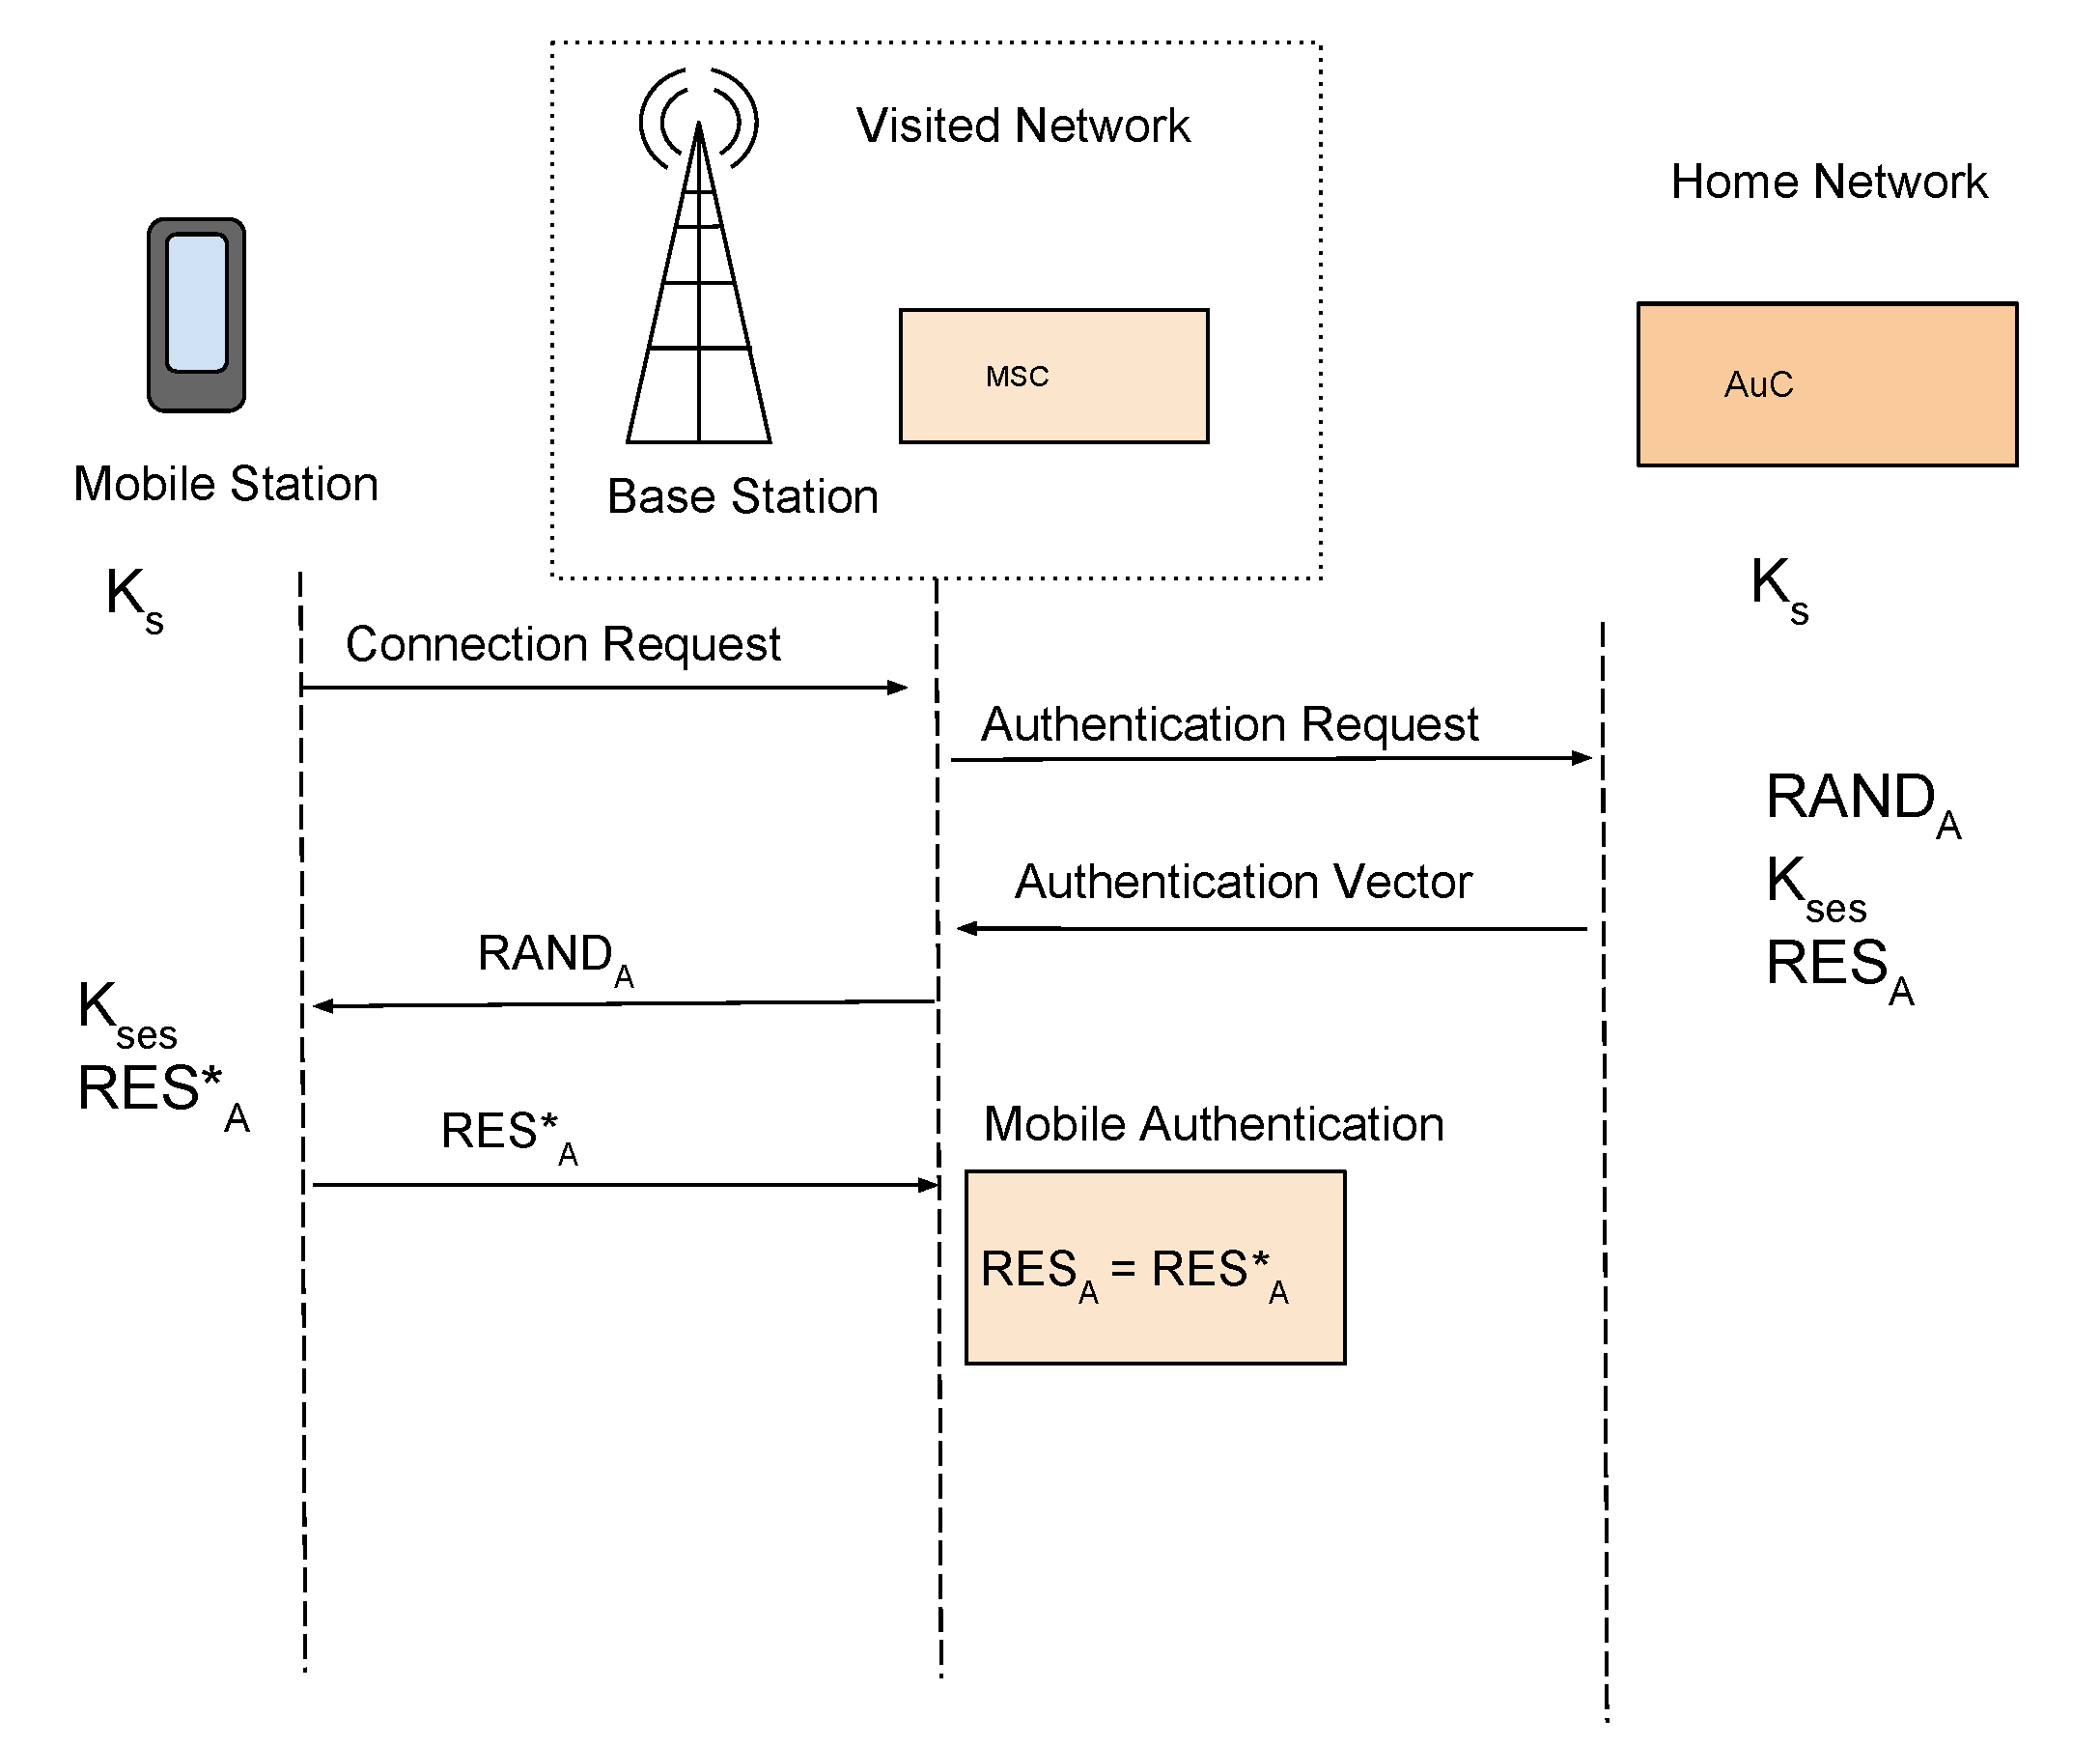
\includegraphics[width=.9\textwidth, height=.85\textheight]{Images/GSMAuthentication3.pdf}

  \end{center} 
\end{frame}
\begin{frame}
% add hidden frames, introduce requests one at a time
  \frametitle{GSM Authentication}

  \begin{center}
  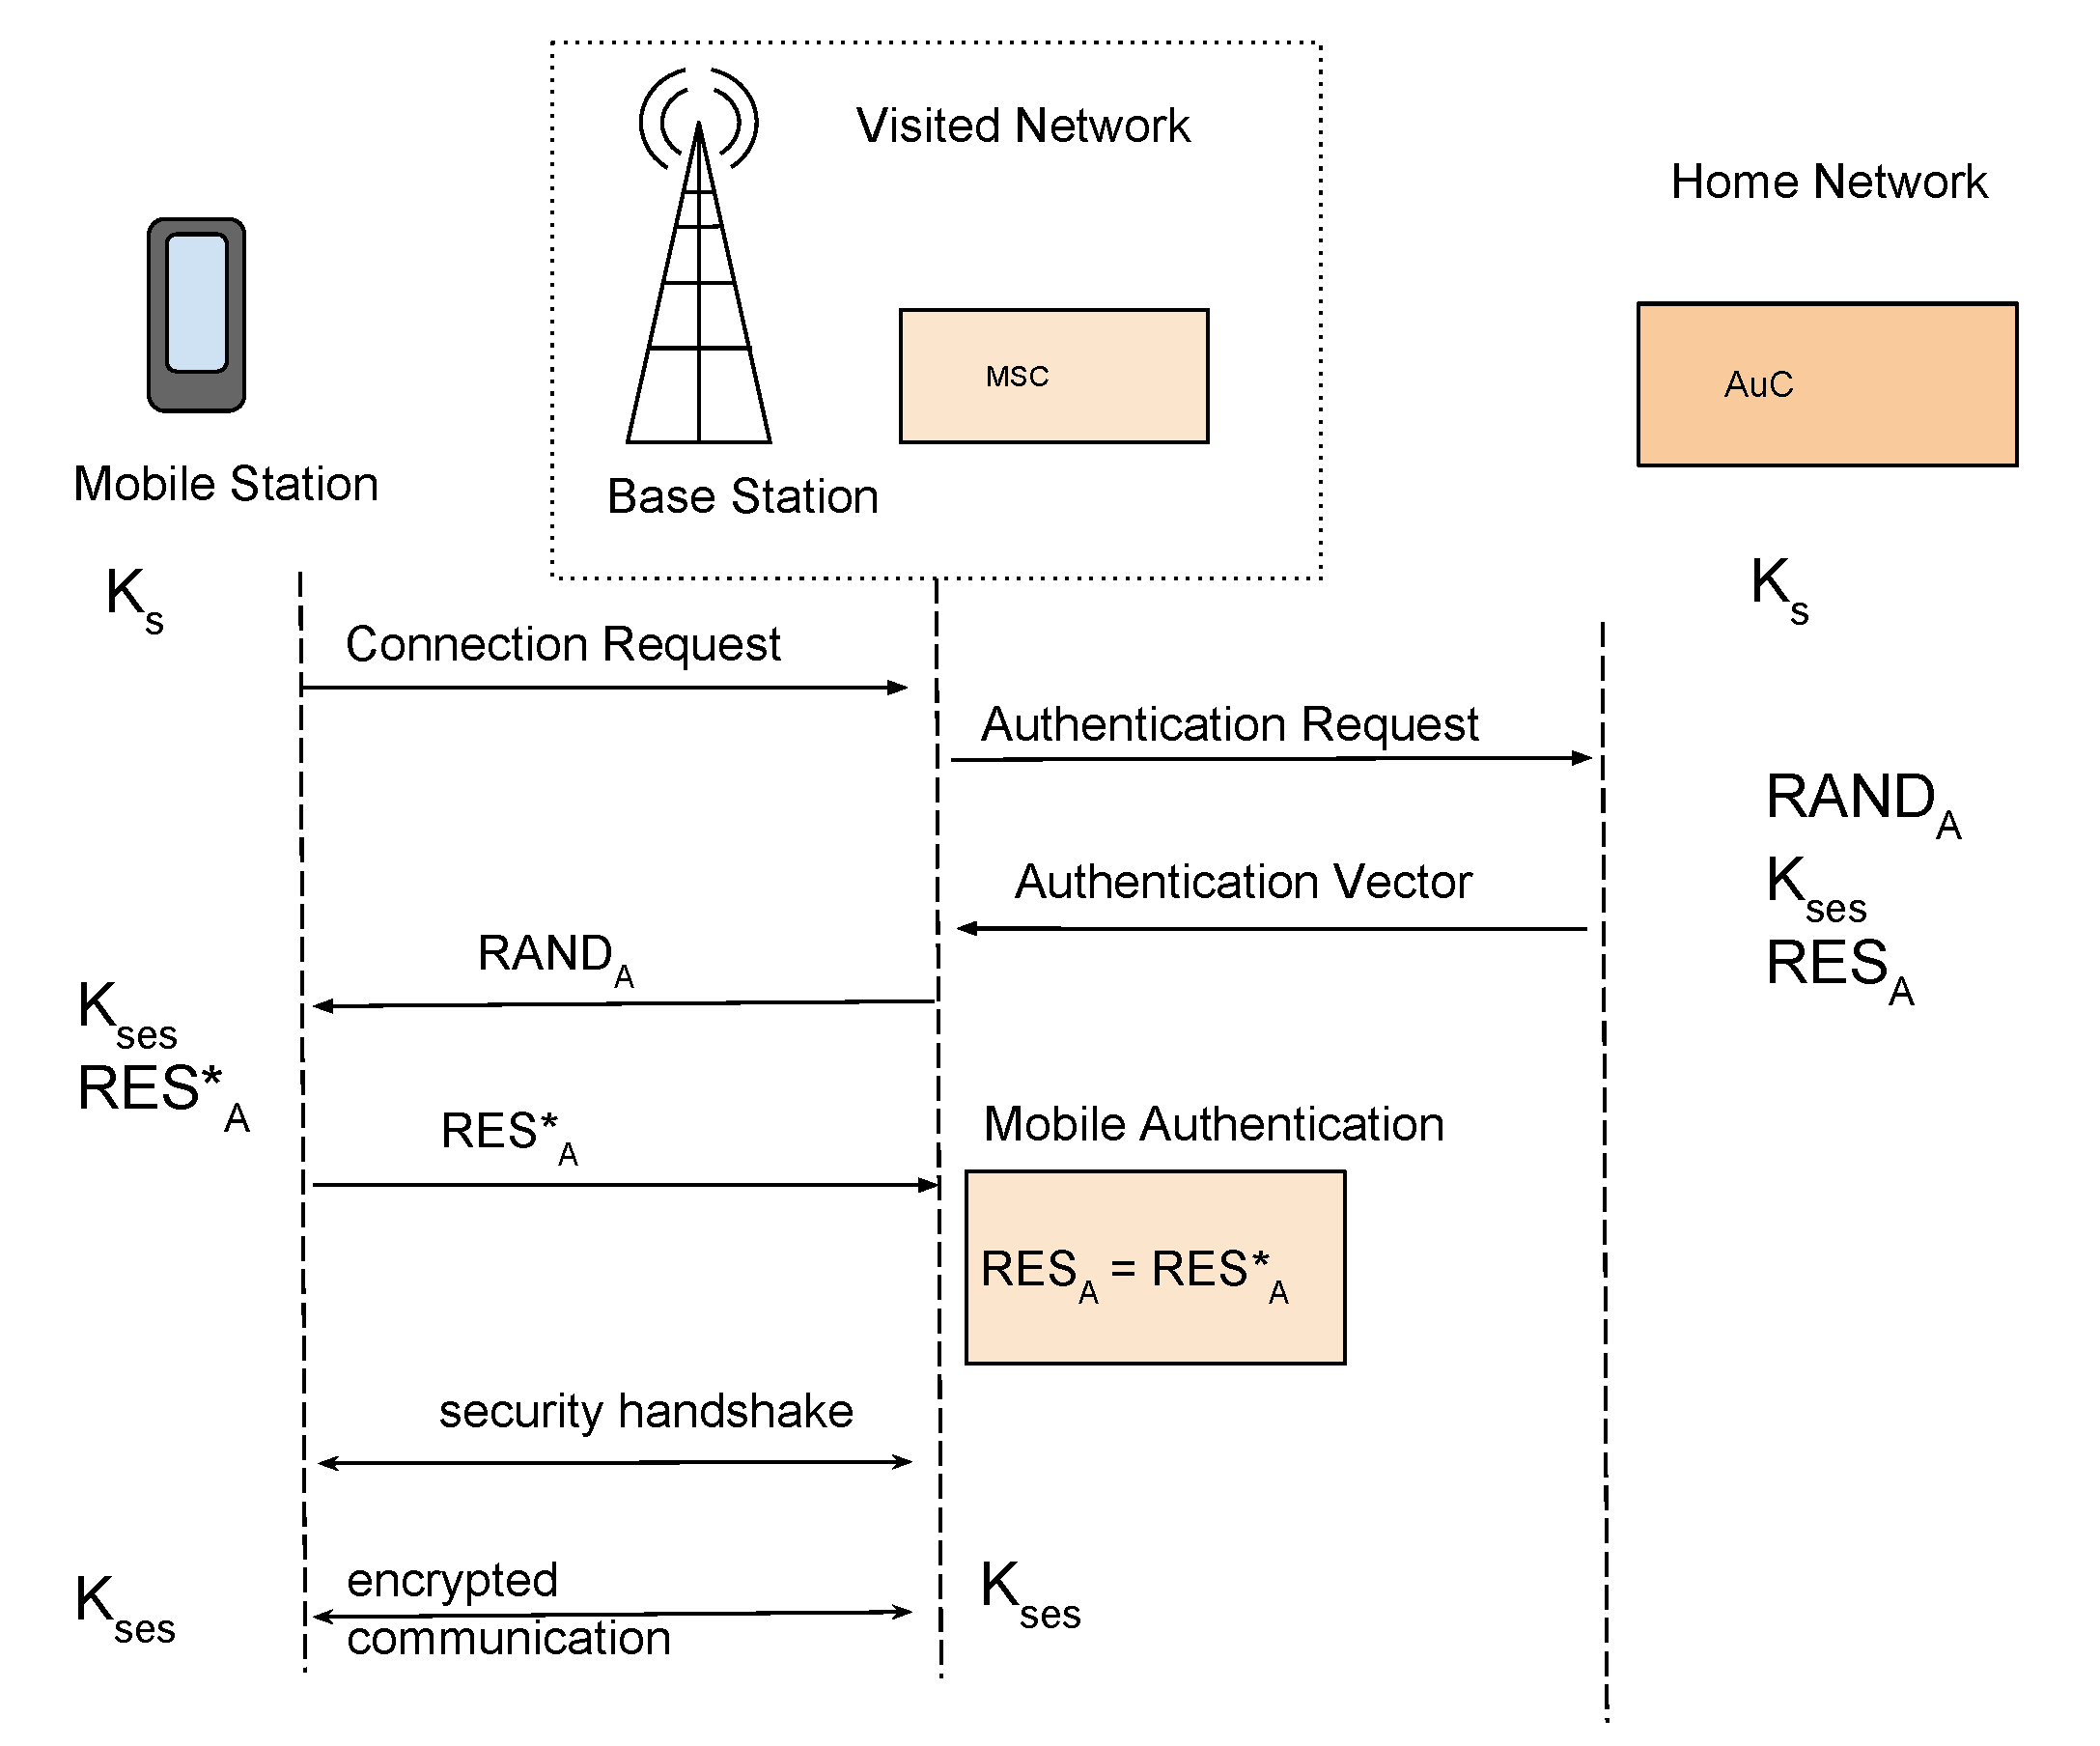
\includegraphics[width=.9\textwidth, height=.85\textheight]{Images/GSMAuthentication4.pdf}

  \end{center} 
\end{frame}
%----------- GSM Man in the middle attack----------------%
\subsection{Man-in-the-middle Attack}
\begin{frame}
	
		\frametitle{Man-in-the-middle Attack}
		\begin{columns}
		\begin{column}[T]{5cm}
		Man-in-the-middle attack is a type of attack in Cryptography where an attacker tricks participants into sending their communications through the attacker.   
		\end{column}
		\column{.5\textwidth}
		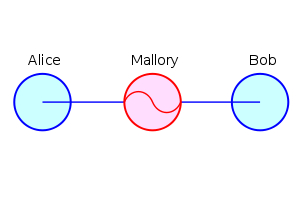
\includegraphics[scale=.45]{Images/MIM.jpg}
		\end{columns}
		\end{frame}
		
		\begin{frame}
	\frametitle{Man-in-the-middle Attack}
		\begin{description}
	\item[1.] Mallory intercepts Alice's message to Bob asking for his public key.\hfill\\
	$Alice$: ``Hi Bob, it's Alice send me your key" $\rightarrow$ $Mallory$
	\item[2.] Mallory relays the message to Bob; Bob cannot tell if the message is really from Alice \hfill\\
	 $Mallory$ ``Hi Bob, it's Alice send me your key" $\rightarrow$ $Bob$ 	
	\item[3.]Bob responds with his key \hfill\\
	$Mallory$ $\leftarrow$[key$_{bob}$]  $Bob$
	\end{description}
	\end{frame}
	\begin{frame}
	\frametitle{Man-in-the-middle Attack}
	\begin{description}
	
	\item[4.] Mallory replaces Bob's key with her own, relays this to  Alice, claiming that it is Bobs key\hfill\\
	$Alice$ $\leftarrow$[key$_{Mallory}$] $Mallory$
	\item[5.]
	Believing communication is secure Alice sends Bob a message believing only he can read it. \hfill\\
	$Alice$ ``send \$2000 to account 2034"[key$_{Mallory}$] \\
	$~\quad\quad\quad\quad\rightarrow$ $Mallory$
	\item[6.] Because the message is encrypted with Mallory's key, Mallory can decrypt it, read and modify this message if she so desires, reencrypt it with Bob's key and Bob forward it to Bob who believes it is a secure message from Alice. \hfill\\
	$Mallory$ ``send \$2000 to account 1099"[key$_{Bob}$] $\rightarrow$ $Bob$
	\end{description}	
\end{frame}
		% add man in the middle attack example		
%-----------UMTS Authentication-----------------%
	\begin{frame}
	\frametitle{UMTS Authentication}
  \begin{center}
  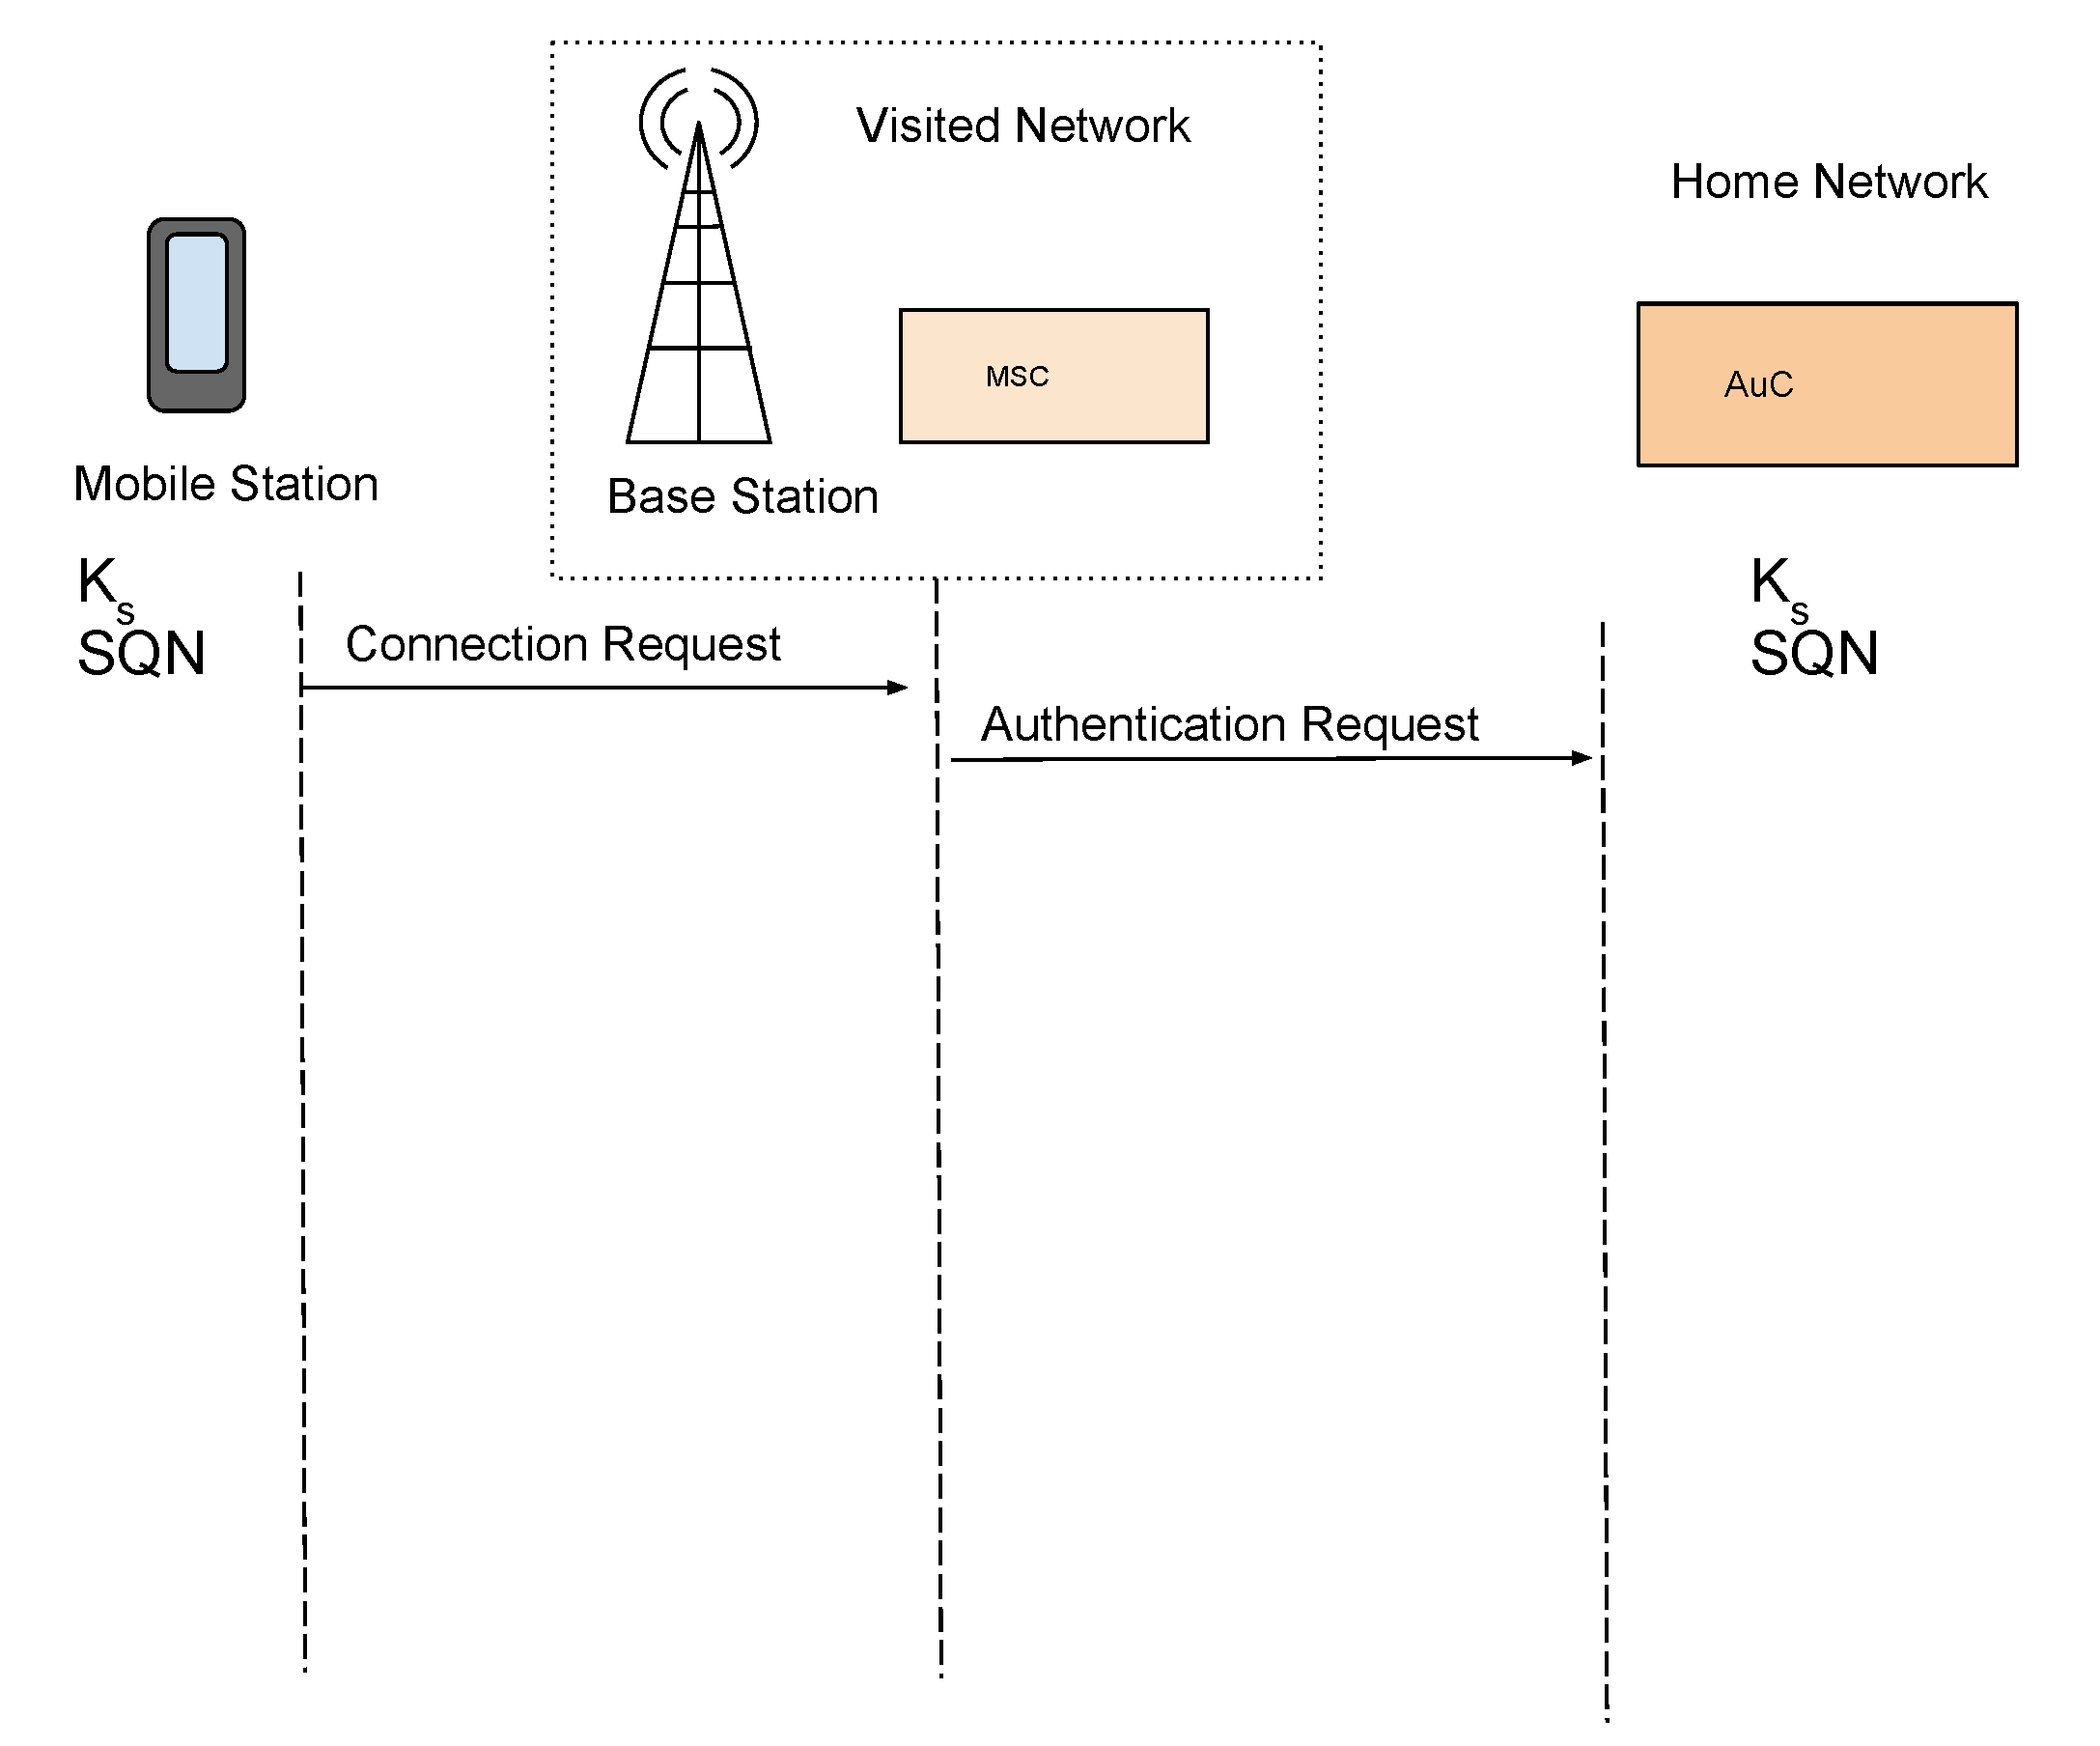
\includegraphics[width=.9\textwidth, height=.85\textheight]{Images/UMTSAuthentication1.pdf}

  \end{center} 
	\end{frame}
	\begin{frame}
	\frametitle{UMTS Authentication}
  \begin{center}
  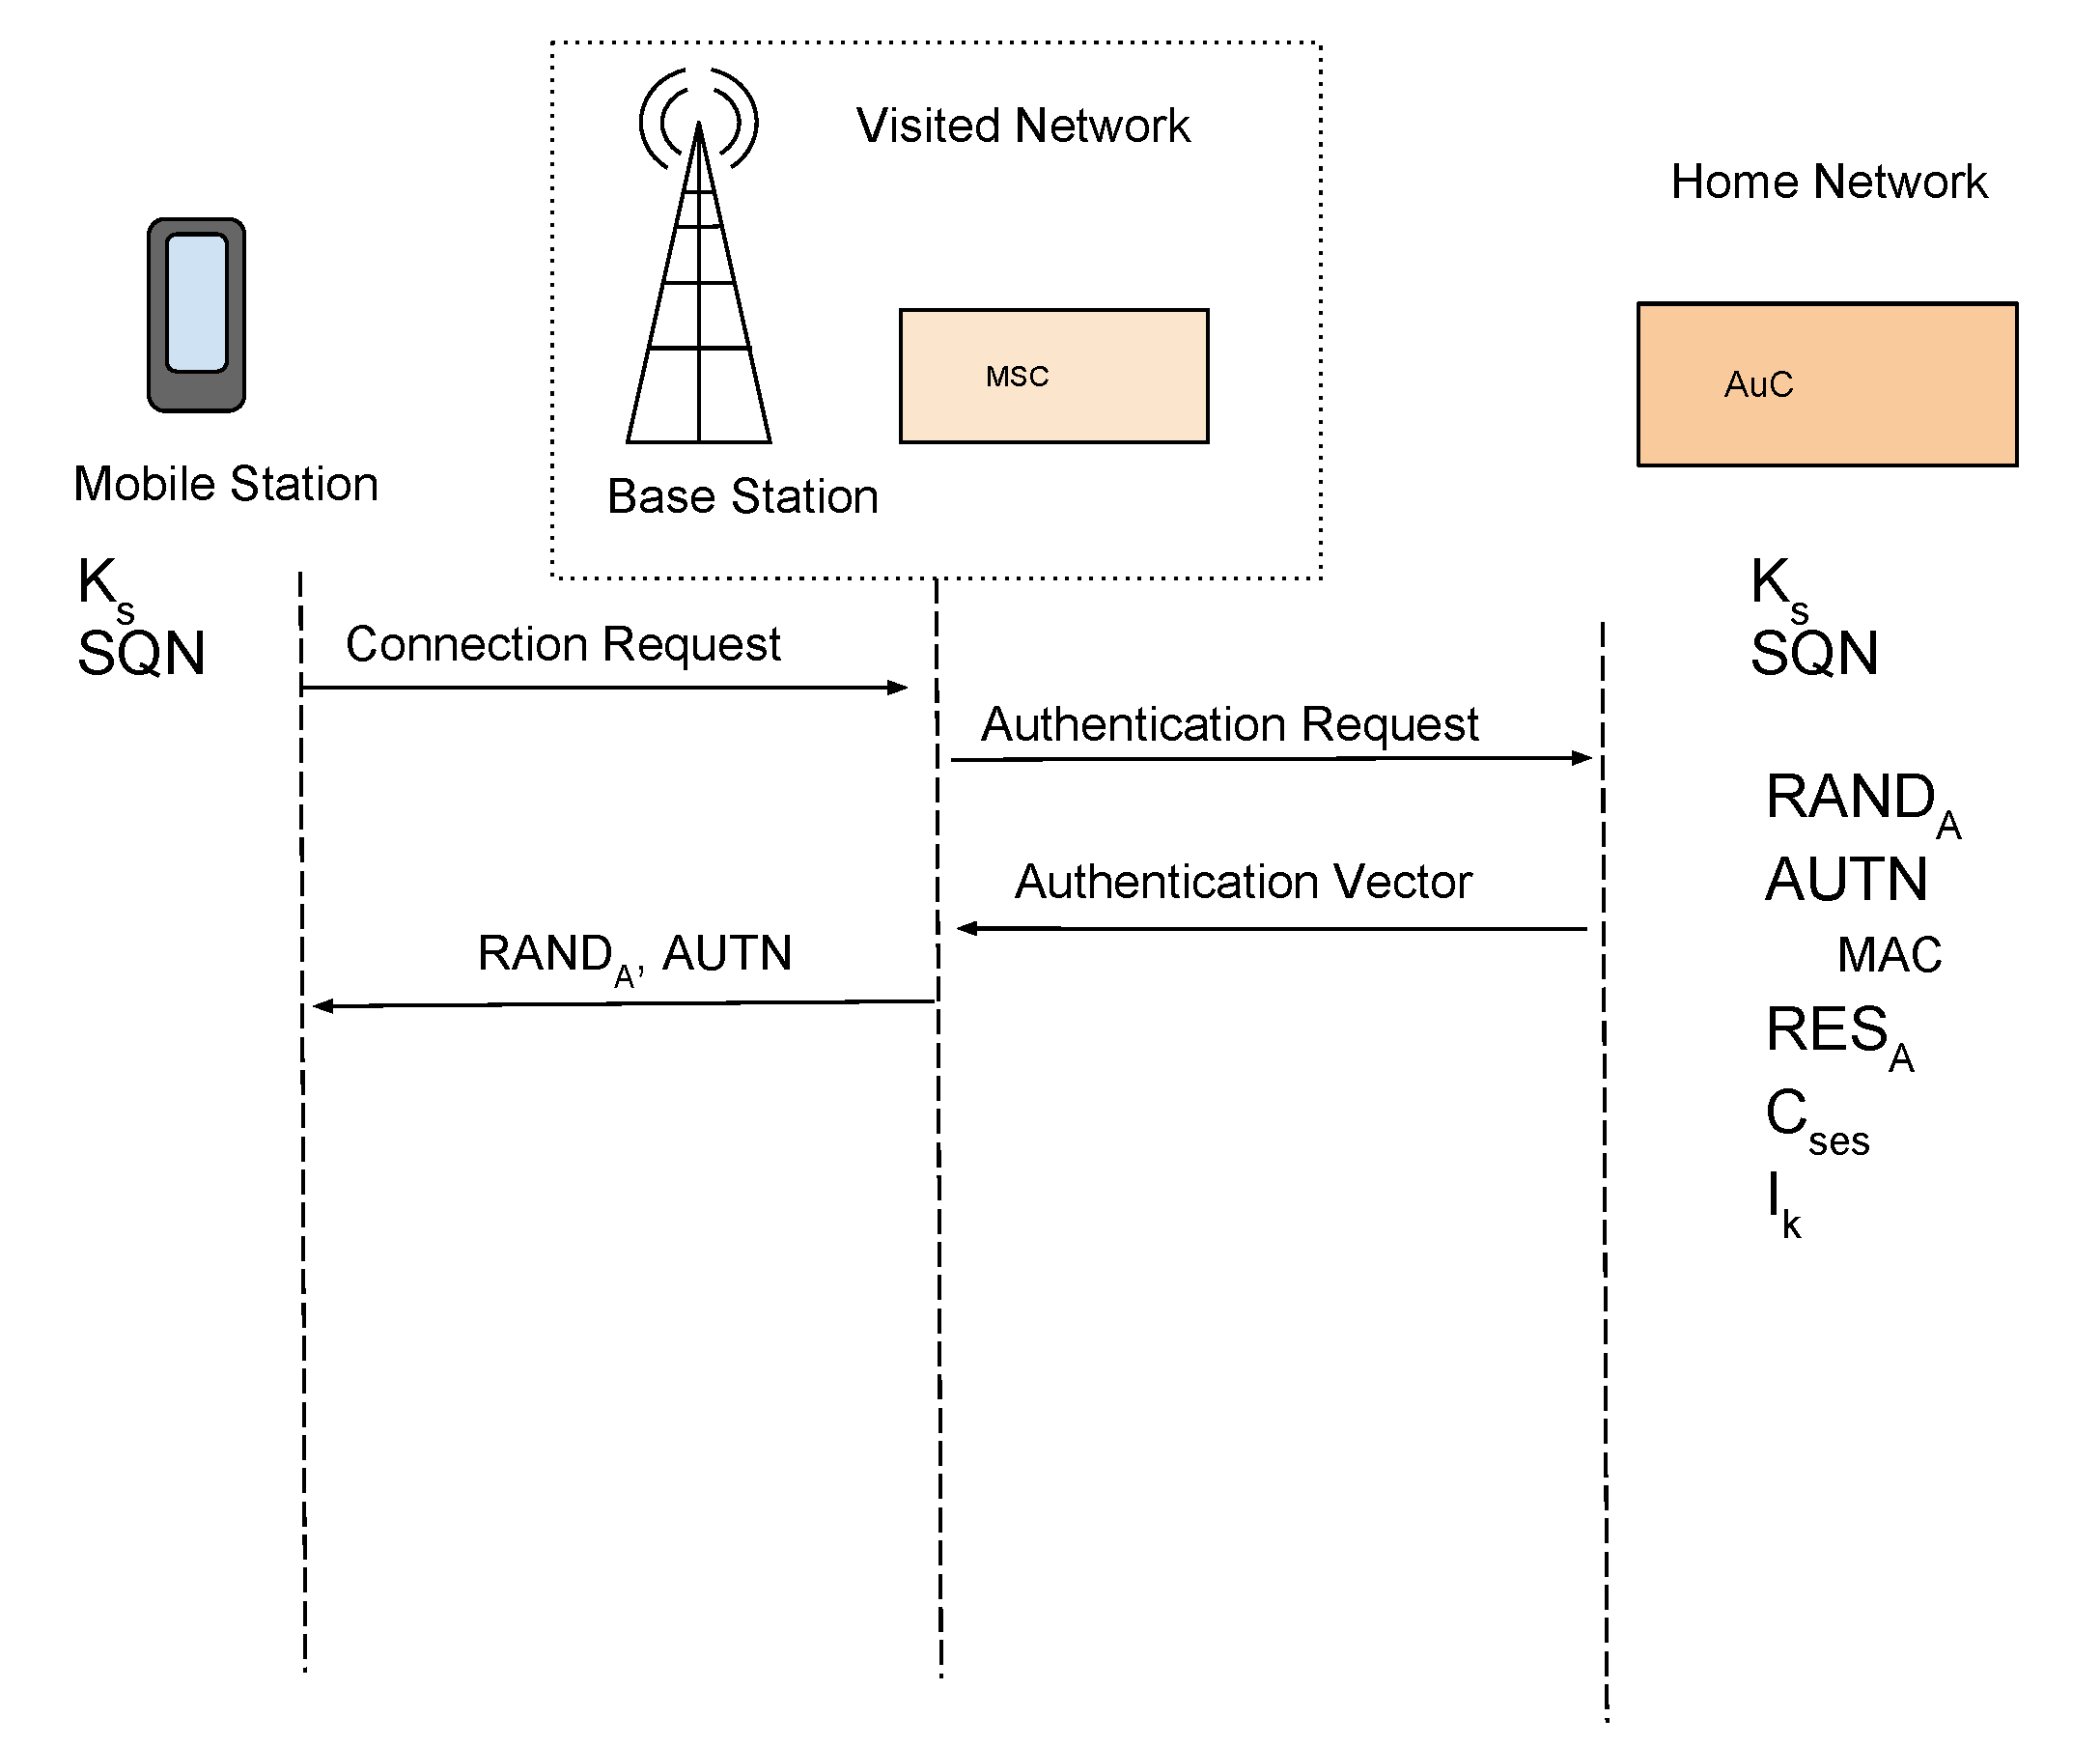
\includegraphics[width=.9\textwidth, height=.85\textheight]{Images/UMTSAuthentication2.pdf}

  \end{center} 
	\end{frame}
	\begin{frame}
	\frametitle{UMTS Authentication}
  \begin{center}
  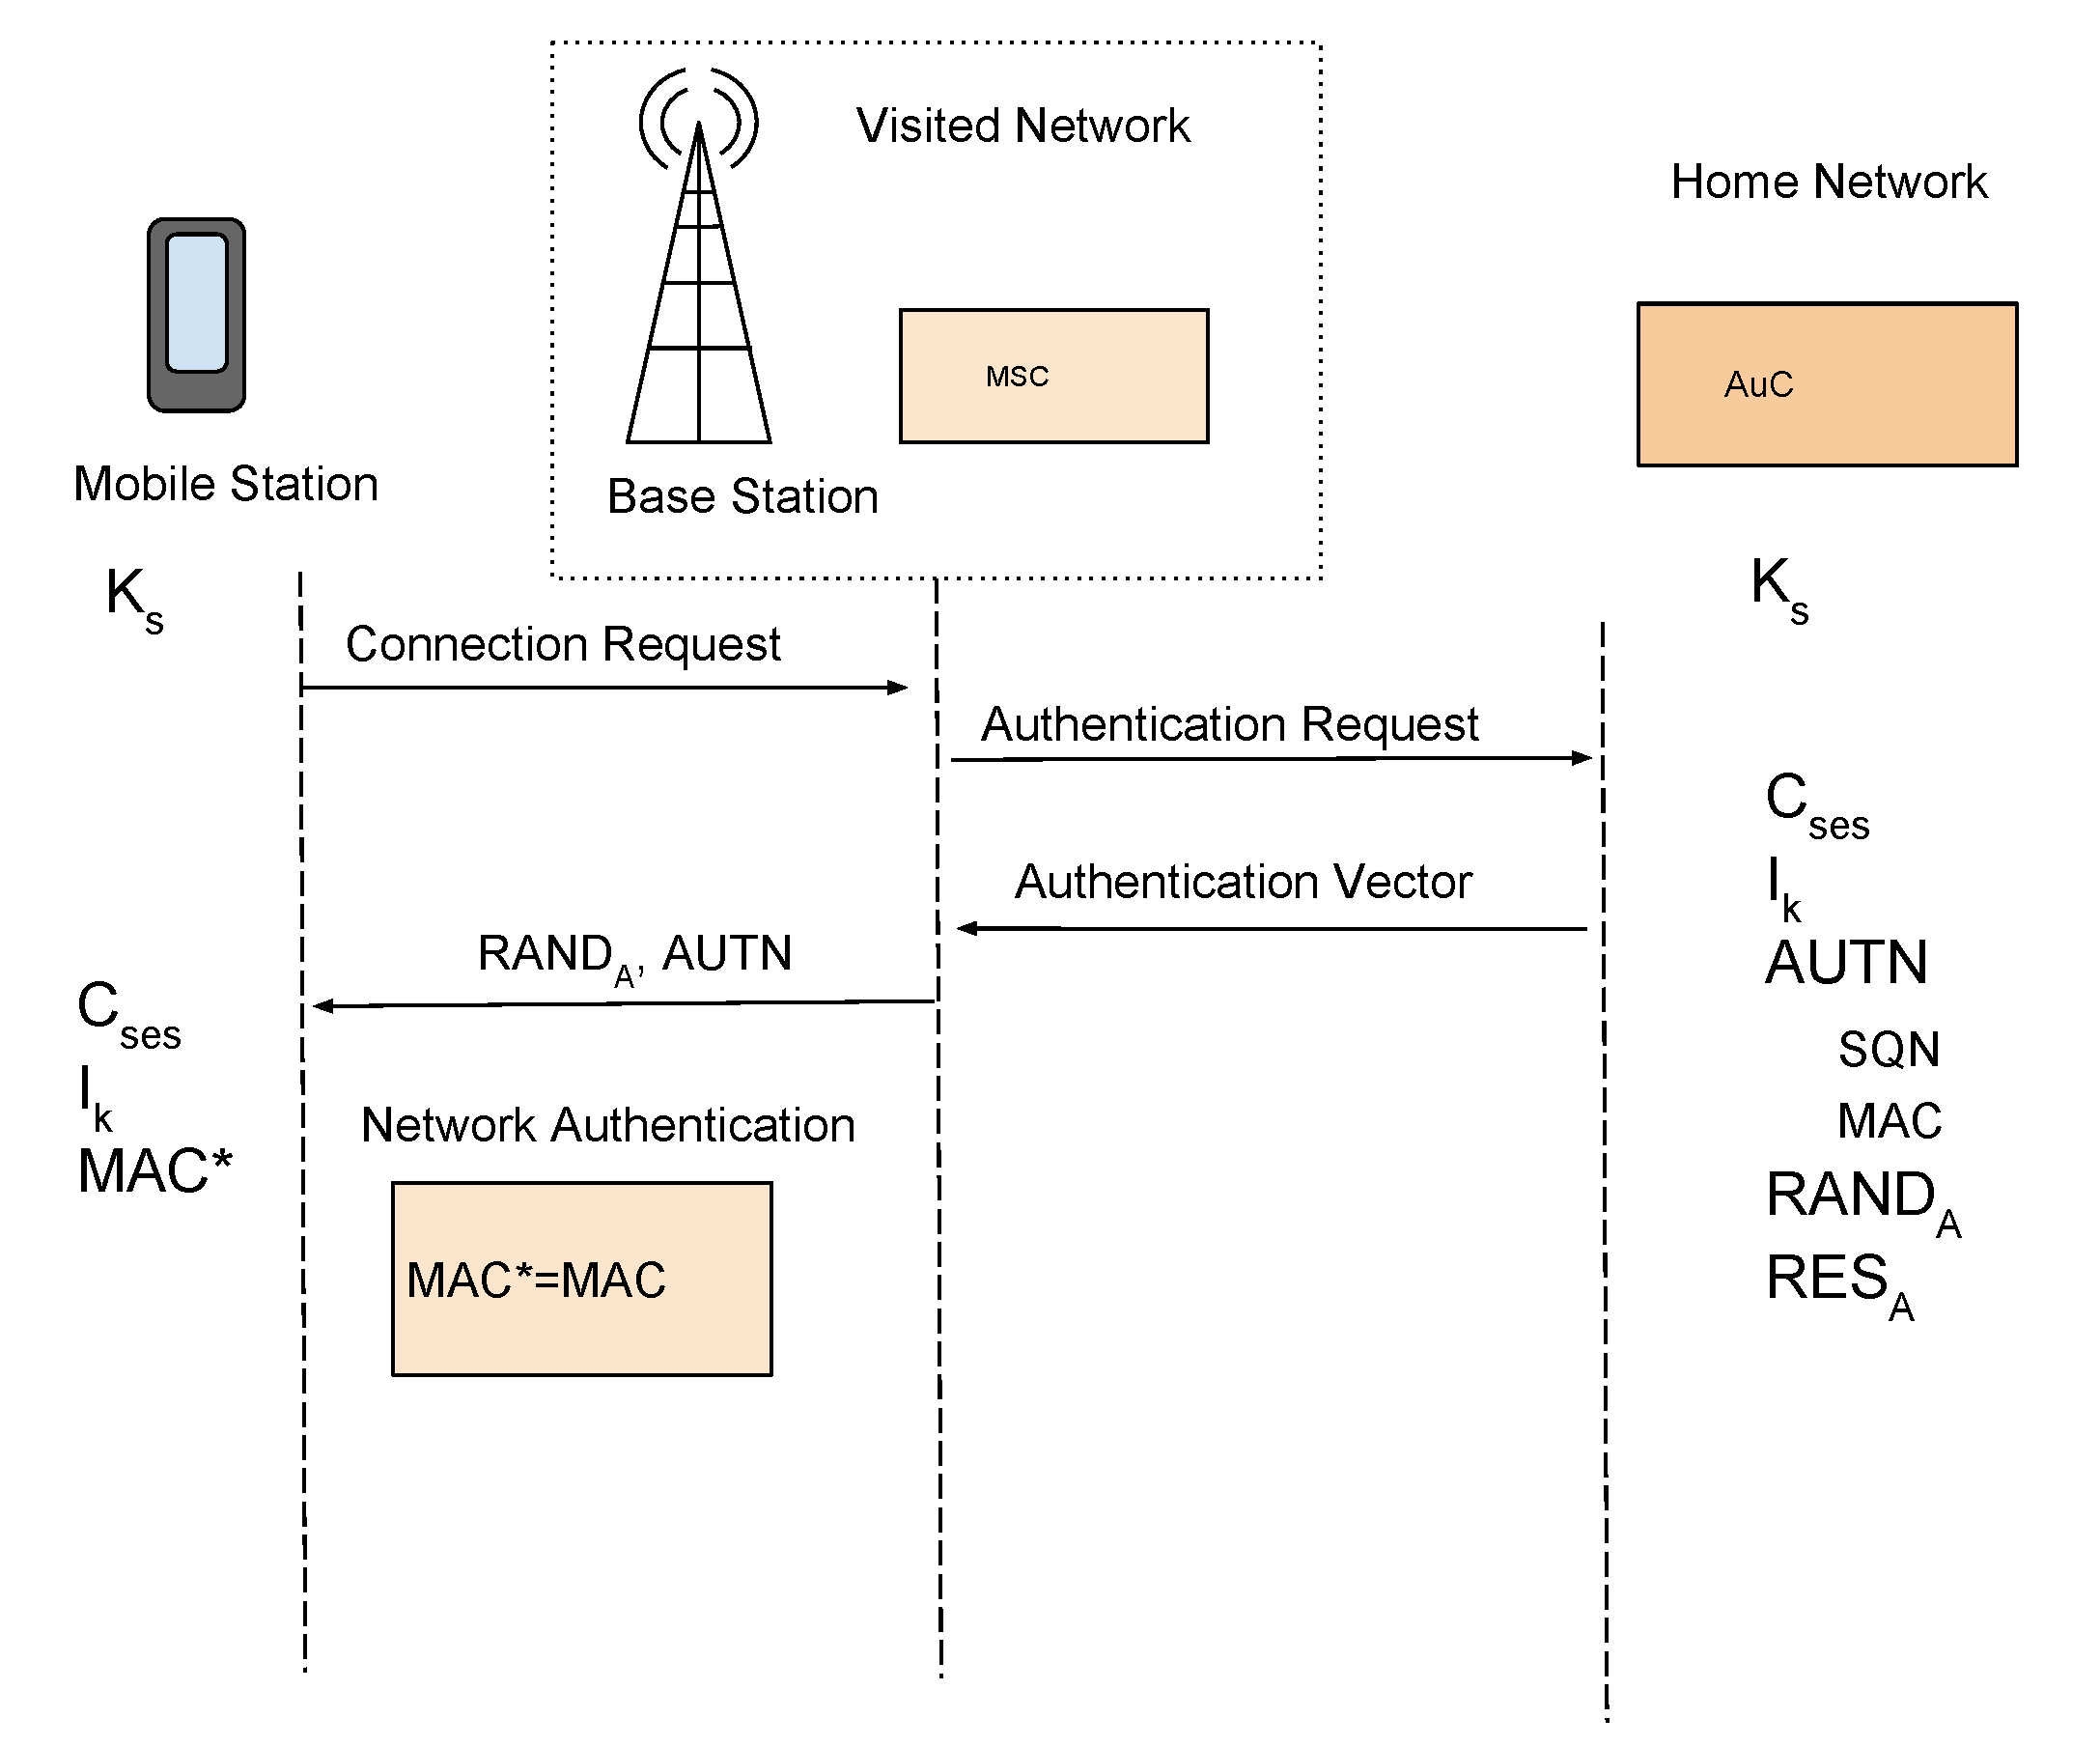
\includegraphics[width=.9\textwidth, height=.85\textheight]{Images/UMTSAuthentication3.pdf}

  \end{center} 
	\end{frame}
\subsection{GSM and UMTS Inter-working Networks}
\begin{frame}
	\frametitle{Transitional Networks}
	Move to after introduce gsm
	 bullet points?\\
		There are transitional periods between old and new technologies such as GSM and UMTS are required as old infrastructure and devices are replaced with the new. During these periods both old and new technologies will need to be able to successfully interact with one another.
		\\2011 survey where 2G devices had around 90\% population coverage where as 3G only had 45\%
\end{frame}

	\begin{frame}
	
	\frametitle{Inter-working networks GSM and UMTS Hand Over}
	
	In order for GSM and UMTS systems to work all UMTS systems must be capable of performing GSM communication this includes a need for a handover. Handover refers to when a mobile is in the middle of preforming communication when it needs to switch to a new base station. For encryption this means there needs to be ways of transforming 128 bit UMTS keys into the 64 bit GSM keys and vise versa\\ 
	
	
	\end{frame}
	\begin{frame}
		\frametitle{Conversion}
		\textbf{UMTS to GSM}
		\begin{equation}
			\label{C_3}
			\mathit{K_{ses} = c_{3}(I_{K},C_{ses}) = C_{ses1} \oplus 					C_{ses2}\oplus I_{K1} \oplus I_{K2}}
		\end{equation}\\
		\textbf{GSM to UMTS}
		\begin{equation} 
			\label{C_4}
			\mathit{C_{ses} = c_{4}(K_{ses}) = K_{ses} \| K_{ses}}
		\end{equation}\\

		\begin{equation}
			\label{C_5}
			\mathit{I_{K} = c_{5}(K_{ses}) = K_{ses1}\oplus K_{ses2}\|					K_{ses}\|K_{ses1}\oplus K_{ses2}}
		\end{equation}
	
\end{frame}	
		
\begin{frame}
	\frametitle{GSM Man-in-the-middle weakness in UMTS}
	\begin{itemize}
	\item[1]Meyer et al describe a Man-in-the-middle attack against UMTS using GSM's man-in-the-middle weakness.
	\item[2]An attacker sets up a dummy base station tricks a UMTS device into connecting to it
	\item[3]Attacker relays messages between mobile device and the legitimate network
	\item[4]During Hand Shake procedure the attacker selects A5/0 algorithm
	\end{itemize}
	
	
	% refer back to GSM authentication diagram ?
\end{frame}
\subsection{Solution}
\begin{frame}


\frametitle{Protecting UMTS from GSM Man-in-the-middle attack}
 Additional authentication and key generation step would be performed before a handover procedure.\\
 Protects broken session keys from being transformed and carried over after the handover.
\end{frame}
\section{Application Security Threat}

%-------------------   Applications   -------------------------------%
	\subsection{Applications}
		\begin{frame}
		\frametitle{Applications (Apps)}
		\begin{itemize}
		\item Applications or Apps are software designed to run on mobile devices 
		\item Apple reported 40 billion app downloads in first quarter of 2013 
		\item Apps pose a security threat as they can have access to both user and the system such as to access contacts and send messages.
		\end{itemize}
		\end{frame}
		\begin{frame}
		\frametitle{Application Threat keyboard Key-logger}
		\begin{itemize}
		\item Mohsen et al. describes the possibility of an Android keyboard application that acts as a key-logger
		\item A key-logger is a device or piece of software that records key strokes
		% which are then sent to the attacker%
		\item user names, passwords and credit card numbers  
		\end{itemize}
		 %
		 % In order for an application to collect and send such information it needs a number of permissions
		 %
		\end{frame}
		\begin{frame}
		\frametitle{Application Permissions in Android}
		%permissions are chategorized into two groups normal and dangerous
		%Every App needs to specify its permissions in AndroidManifest.xml file, this 	        %file is read by the system and then 
\begin{center}			
			\begin{columns}[t]
			\begin{column}[T]{5cm}
			 \textbf{Normal permissions}
			% permissions are those that are not considered harmfull to 
			%the user or the system these are granted automatically
			\end{column}
			\begin{column}[T]{5cm}
			\textbf{Dangerous permissions}
			% permissions considered harmfull to the user or the system
			% these must be oked by the user. Most of the time a user 
			%either doesn't know the dangers of these permissions or more 
			%likely doesn't really care 
			Example would be the ability to access user data, send SMS messages, access camera.
			\end{column}
				
			\end{columns}
			\end{center}
		\end{frame}
		
	\subsection{Solution}
		\begin{frame}
		\frametitle{KBS Checker}
		%Mohsen et al. designed a software system called KBS Checker.
		%KBS Checker reads through all the XML permission files of 		
		%installed apps, looking for combinations of permissions that
		% could potentially indicate a key-logging app.
		%This same Idea could be applied to detect malicious apps and 
		%inform users of this threat.
		\begin{columns}[t]
		\begin{column}{.45\textwidth}
		\textbf{KBS Checker}
		\begin{itemize}
		\item Reads app Permissions
		\item Looks for dangerous combinations of permissions
		\item Warns user with the app's name and the threat it could pose
		\end{itemize}
		\end{column}
		\begin{column}{.45\textwidth}
			\textbf{KBS Checker}
			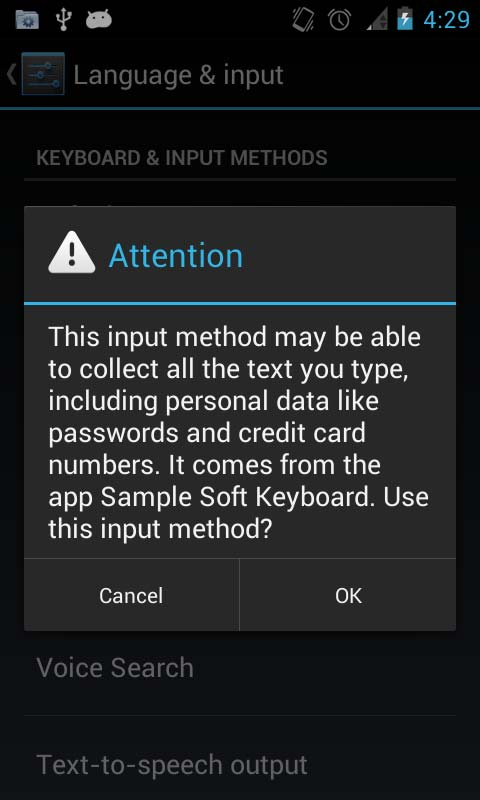
\includegraphics[width = \textwidth]{Images/KBSChecker.png} 
		\end{column}
		\end{columns}
		\end{frame}
		
		
	% ------     Ranged Side-channel Attack      ---------%		
		
\section{Ranged Side-channel Attack}
        \begin{frame}
		\frametitle{Ranged Side channel}
		\begin{columns}
		\begin{column}{.45\textwidth}
		Kenworthy et al. described an attack using inexpensive radio equipment to capture and analyze electro magnetic (EM) to perform a ranged side-channel attack.
		\end{column}
		\begin{column}{.45\textwidth}
		
			 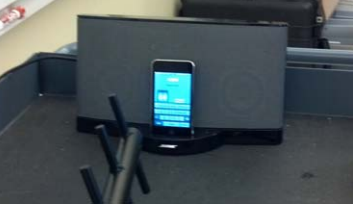
\includegraphics[width=\textwidth]{Images/antennaWithDevice.png}
			 \linebreak
			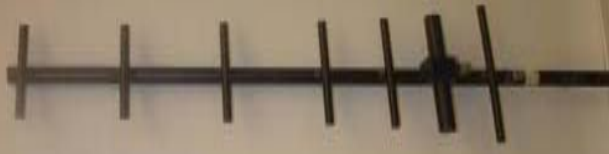
\includegraphics[width=\textwidth]{Images/antenna.png} 
			
		\end{column}
		\end{columns}
		% Intro for the researchers and about their
		% Ranged side channel attack 
		%  and how using basic equipment they can			
		% pick up the EM(Electro Magnetic) radiation produced from the 
		% device during when it is preforming encryption
		%
		% -crypto procedures require quite a bit of computation -> 		  
		%requiring mor  power and thus leades to fluctuations in EM 
		%Strength
		\end{frame}
	\subsection{Side channel attack}
		\begin{frame}
		\frametitle{What is a Side channel attack?}
			\begin{itemize}
			\item Cryptographic attack like man-in-the middle\\
			\item Uses physical properties of the machine doing the encryption revealing by-products of the encryption process.  \\
			\item physical properties can include things such as cpu heat, power consumption or even sound.
		\end{itemize}
			% Another cryptographic attack like MIM
			% Uses physical properties of a machine while its preforming 
			%encryption
			% Heat, Sound, Power 
			% uses these properties to exploit characteristics of a chiper 			%to derive the key
			% usually invasive requiring direct access to the device
		\end{frame}
		\begin{frame}
		\frametitle{RSA}
		\begin{columns}[c]
		\begin{column}{.45\textwidth}
		\textbf{RSA}
		 \begin{itemize}
		 \item Commonly used asymmetric cipher used for key establishment
		 \item Uses Square and Multiply method for more efficient modular exponentiation of large positive numbers.
			\end{itemize}
		 \end{column}
		 
		 \begin{column}{.45\textwidth}
		 \textbf{Square and Multiply}
		 \[x^n = \left\{
  \begin{array}{lr}
    x(x^2)^{\frac{n-1}{2}} &  \text{: if n is odd} \\
    (x^2)^{\frac{n}{2}} & \text{: if n is even}
  \end{array}
\right.
\]
		 \end{column}
		 \end{columns}
		% Commonly used Assymetric cryptographic algorithm
		% using large prime numbers. Utalizes square and multiply method 
		% for faster computations
		%
		% Show square and multiply method
		%
		% Example RSA attack 
		\end{frame}
		\begin{frame}
		  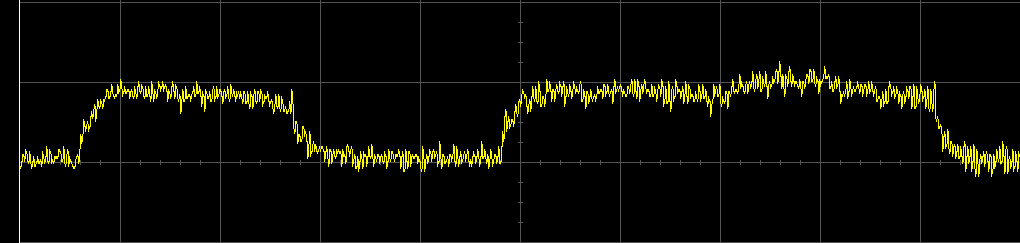
\includegraphics[width= \textwidth]{Images/Power_attack.png} 
		\end{frame}
	\subsection{Side channel through EM}
		
		\begin{frame}
		\frametitle{Findings}
		\begin{columns}[T]
		\begin{column}{.45\textwidth}
		\textbf{Findings}
		\begin{itemize}
		\item tested on multiple os and devices
		\item tested multiple algorithms
		\end{itemize}
		\textbf{Solution}
		\begin{itemize}
		\item add noise to RSA
		\item Bulk encryption
		\end{itemize}
		 
		
		\end{column}
		\begin{column}{.45\textwidth}
		\textbf{RSA EM Attack}
		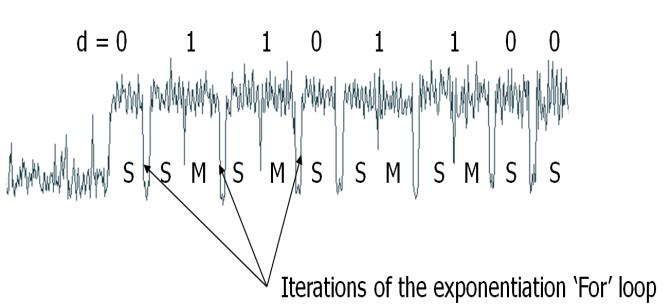
\includegraphics[scale=.3]{Images/RSA.jpg}
		\end{column}
		\end{columns}
		% Tested this on multiple devices with different OSs
		% Using a number of different ciphers
		% were able to desern keys of ciphers 
	
		
			% add noise during cryptographic computations
			
		\end{frame}
\section{Conclusion}
	\begin{frame}
		\frametitle{Conclusion}
		\end{frame}	
		
		\begin{frame}
		\frametitle{Questions}
			\begin{center}
			\Huge Questions?
			\end{center}
		\end{frame}	
		\begin{frame}
		\frametitle{References}
		\end{frame}

\end{document}


